\chapter{Photosynthesis and Autotrophy}\label{ch:b1:photosynthesis}

Every gram of carbon in the rabbit, the oak, the reader and this page
was once carbon dioxide in the air, and was fixed into sugar by a
\omterm{def:b1:flowering-plant-organization:organs}{leaf} --- or by an alga, or a cyanobacterium --- using the energy of
sunlight. The reaction, six $\mathrm{CO_2}$ and six water to one
glucose and six oxygen, is uphill by \qty{2870}{kJ/mol}; a \omterm{def:b1:flowering-plant-organization:organs}{leaf} runs
it by splitting water with light, storing the electrons on NADPH and
the energy on \omterm{def:b1:water-small-molecules:atp}{ATP}, and spending both in a cycle that builds sugar. This
chapter describes the \omterm{def:b1:photosynthesis:chloroplast}{chloroplast}, the pigments and the \omterm{prop:b1:photosynthesis:lightreactions}{light
reactions} that make \omterm{def:b1:water-small-molecules:atp}{ATP} and NADPH, the \omterm{def:b1:photosynthesis:fixation}{Calvin cycle} that fixes carbon,
the leak called photorespiration and the two designs that seal it, and
what \omterm{def:b1:photosynthesis:autotrophy}{autotrophy} is in general.

\section{The chloroplast and its pigments}

\begin{definition}[Chloroplast]\label{def:b1:photosynthesis:chloroplast}
The \emph{chloroplast}\index{chloroplast} is a lens-shaped \omterm{def:b1:cell-unit-of-life:prokeuk}{organelle}
\qtyrange{3}{10}{\micro m} long bounded by two envelope membranes; its
interior, the \emph{stroma}\index{stroma}, holds the \omterm{def:b1:enzymes:enzyme}{enzymes} of carbon
fixation, \omterm{def:b1:carbohydrates:polysaccharide}{starch} grains, ribosomes and a circular \omterm{def:b1:nucleic-acids:chain}{DNA}; within the
stroma a third membrane system, the \emph{thylakoids}\index{thylakoid},
forms flattened sacs stacked into \emph{grana} and connected by
lamellae, enclosing one continuous \emph{thylakoid lumen}. The \omterm{prop:b1:photosynthesis:lightreactions}{light
reactions} take place in the thylakoid membrane; carbon fixation in the
stroma. A \omterm{def:b1:flowering-plant-organization:organs}{leaf} \omterm{def:b1:cell-unit-of-life:cell}{cell} holds \qtyrange{20}{100}{} \omterm{def:b1:eukaryotic-cell:plastid}{chloroplasts}; a square
millimetre of \omterm{def:b1:flowering-plant-organization:organs}{leaf}, half a million.
\end{definition}

\begin{omfigure}
\begin{tikzpicture}
  \node[anchor=south west, inner sep=0] (img) at (0,0)
    {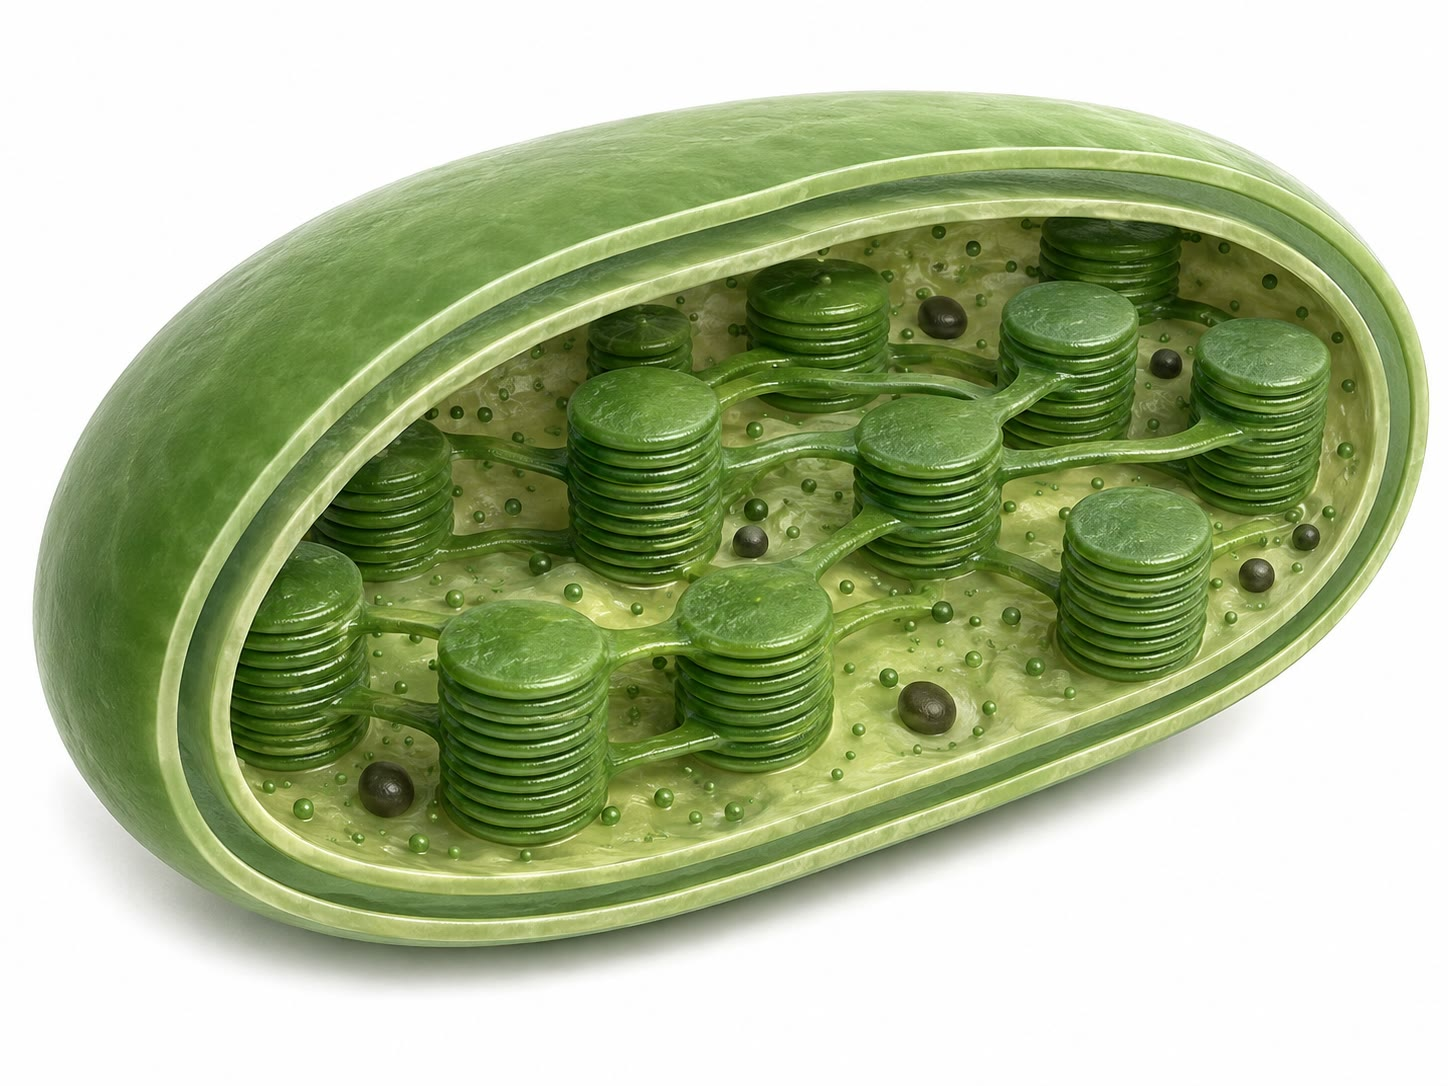
\includegraphics[width=0.56\linewidth]{images/book3/ai/fig-chloroplast-cutaway.jpg}};
  \begin{scope}[x={(img.south east)}, y={(img.north west)},
      every node/.style={font=\small}]
    \draw[omDef, thick] (0.12,0.50) -- (-0.03,0.66) node[left, align=right] {two envelope\\ membranes};
    \draw[omDef, thick] (0.48,0.60) -- (0.48,1.08) node[above] {granum: a stack of thylakoids};
    \draw[omDef, thick] (0.62,0.52) -- (1.03,0.62) node[right] {stroma lamella};
    \draw[omDef, thick] (0.35,0.24) -- (-0.03,0.16) node[left] {stroma};
    \draw[omDef, thick] (0.86,0.50) -- (1.03,0.40) node[right] {starch grain};
  \end{scope}
\end{tikzpicture}

{\small A \omterm{def:b1:photosynthesis:chloroplast}{chloroplast} cut open. Two envelope membranes around the
\omterm{def:b1:photosynthesis:chloroplast}{stroma}; inside, stacks of \omterm{def:b1:photosynthesis:chloroplast}{thylakoids} (grana) connected by lamellae and
enclosing a single lumen. Light is captured in the \omterm{def:b1:photosynthesis:chloroplast}{thylakoid} membrane
and sugar is made in the \omterm{def:b1:photosynthesis:chloroplast}{stroma}.}
\end{omfigure}

\begin{definition}[Photosynthetic pigments]\label{def:b1:photosynthesis:pigments}
\emph{Chlorophyll}\index{chlorophyll} $a$ and $b$ are porphyrin rings
around a magnesium atom with a long hydrophobic tail anchoring them in
the \omterm{def:b1:photosynthesis:chloroplast}{thylakoid} membrane; they absorb blue (\qtyrange{430}{450}{nm}) and
red (\qtyrange{640}{680}{nm}) light and reflect green.
\emph{Carotenoids}\index{carotenoid} (\omterm{def:b1:lipids:steroids}{isoprenoids}, \cref{ch:b1:lipids})
absorb blue-green light and pass the energy to chlorophyll, and
protect it by quenching excess excitation. A few hundred pigment
molecules, held on \omterm{def:b1:proteins:peptide}{proteins} as an \emph{antenna} (light-harvesting
complex), funnel the energy of every absorbed photon to one special
pair of chlorophyll $a$ molecules, the \emph{reaction centre}, where
it is turned into chemistry.
\end{definition}

\begin{omfigure}
\begin{tikzpicture}
\begin{axis}[
  width=0.88\linewidth, height=6.2cm,
  axis x line=bottom, axis y line=left,
  xmin=400, xmax=720, ymin=0, ymax=1.1,
  xlabel={wavelength (\unit{nm})}, ylabel={absorption, or rate (relative)},
  xlabel style={font=\small, at={(axis description cs:0.5,-0.12)}, anchor=north},
  ylabel style={font=\small},
  tick label style={font=\small}, xtick={400,450,500,550,600,650,700}, ytick={0,0.5,1},
  legend style={font=\small, at={(0.5,0.98)}, anchor=north, draw=none},
  clip=false,
]
\addplot[very thick, omDef, domain=400:720, samples=160] {exp(-((x-430)/18)^2) + 0.85*exp(-((x-662)/14)^2) + 0.05};
\addlegendentry{absorption of chlorophyll $a$}
\addplot[very thick, omExo, domain=400:720, samples=160] {0.7*exp(-((x-455)/20)^2) + 0.5*exp(-((x-645)/14)^2) + 0.05};
\addlegendentry{absorption of chlorophyll $b$}
\addplot[very thick, omProp, domain=400:720, samples=160] {0.75*exp(-((x-470)/25)^2) + 0.05};
\addlegendentry{absorption of carotenoids}
\addplot[very thick, dashed, omThm, domain=400:720, samples=160] {0.9*exp(-((x-440)/30)^2) + 0.35*exp(-((x-520)/50)^2) + 0.85*exp(-((x-660)/22)^2) + 0.1};
\addlegendentry{action spectrum: rate of $\mathrm{O_2}$ release}
\end{axis}
\end{tikzpicture}

{\small Absorption spectra of the three pigment classes and the
action spectrum of photosynthesis (the rate of oxygen release at each
wavelength). The action spectrum follows the \omterm{def:b1:photosynthesis:pigments}{chlorophylls}, filled in
by the \omterm{def:b1:photosynthesis:pigments}{carotenoids} in the blue-green: every pigment that absorbs
contributes.}
\end{omfigure}

\begin{proposition}[The action spectrum follows the pigments]\label{prop:b1:photosynthesis:engelmann}
Photosynthesis is driven by the light the pigments absorb: it is
fastest in red and blue light, weakest in green.
\end{proposition}
\begin{proof}[Evidence]
Engelmann (1882) laid a filament of alga across a spectrum projected
under his microscope and added oxygen-seeking bacteria: they gathered
where the red and blue light fell, not in the green (recalled from the
High School volume). Measured with an oxygen electrode, the rate at
each wavelength gives the action spectrum above, which follows the
absorption of the \omterm{def:b1:photosynthesis:pigments}{chlorophylls}; the excess in the blue-green is the
\omterm{def:b1:photosynthesis:pigments}{carotenoids}' contribution, showing that they pass their energy on.
\end{proof}

\section{The light reactions}

\begin{proposition}[What the light reactions do]\label{prop:b1:photosynthesis:lightreactions}
\index{light reactions}
In the \omterm{def:b1:photosynthesis:chloroplast}{thylakoid} membrane, light energy is used to move electrons from
water to $\mathrm{NADP^+}$ --- uphill, against a redox potential
difference of \qty{1.1}{V} --- and to pump protons into the lumen:
\[
2\,\mathrm{H_2O} + 2\,\mathrm{NADP^+} + 3\,\mathrm{ADP} + 3\,\mathrm{P_i}
\xrightarrow{\ 8\ \text{photons}\ }
\mathrm{O_2} + 2\,\mathrm{NADPH} + 2\,\mathrm{H^+} + 3\,\mathrm{ATP} .
\]
The oxygen released is the oxygen of water, not of carbon dioxide;
the NADPH carries the reducing power and the \omterm{def:b1:water-small-molecules:atp}{ATP} the energy that the
\omterm{def:b1:photosynthesis:fixation}{Calvin cycle} will spend.
\end{proposition}
\begin{proof}[Evidence]
Hill (1937) showed that isolated \omterm{def:b1:eukaryotic-cell:plastid}{chloroplasts} in light release oxygen
in the absence of $\mathrm{CO_2}$ if an artificial electron acceptor
is present: the splitting of water is separable from carbon fixation.
Ruben and Kamen (1941) fed algae water labelled with heavy oxygen and
found the label in the $\mathrm{O_2}$ released, and not when the label
was in the $\mathrm{CO_2}$. Emerson (1957) found that red light of
\qty{700}{nm}, nearly useless alone, and light of \qty{680}{nm}
together gave more than the sum of their separate rates: two
\omterm{def:b1:photosynthesis:zscheme}{photosystems} with different pigments must work in series.
\end{proof}

\begin{definition}[Photosystems and the Z-scheme]\label{def:b1:photosynthesis:zscheme}
\index{photosystem}\index{Z-scheme}
Two \emph{photosystems} sit in the \omterm{def:b1:photosynthesis:chloroplast}{thylakoid} membrane. In
\emph{photosystem II} (PSII, reaction centre P680) an absorbed photon
raises an electron of the special pair to a high energy; the electron
\omterm{def:b1:flowering-plant-organization:organs}{leaves}, and the oxidised P680, the strongest biological oxidant,
takes an electron from water: a manganese cluster splits two water
molecules into $\mathrm{O_2}$, four protons (released into the lumen)
and four electrons, one photon at a time. The electron descends an
\emph{electron-transport chain} --- plastoquinone, the
\emph{cytochrome $b_6f$ complex}, plastocyanin --- and the energy it
loses pumps protons into the lumen. In \emph{photosystem I} (PSI,
P700) a second photon lifts it again, to a potential low enough to
reduce ferredoxin and then $\mathrm{NADP^+}$ to NADPH. Drawn on a
scale of redox potential, the path is a Z: two climbs by light, two
descents by chemistry.
\end{definition}

\begin{omfigure}
\begin{tikzpicture}[font=\footnotesize, >=Stealth, line cap=round,
  st/.style={draw, thick, rounded corners=2pt, inner sep=2pt}]
  % redox potential axis (vertical, more negative up)
  \draw[->, thick] (0,0) -- (0,6.4) node[above, font=\small] {redox potential $E'_0$ (V)};
  \foreach \y/\l in {0.4/{$+1.0$}, 1.9/{$+0.5$}, 3.4/{$0$}, 4.9/{$-0.5$}, 6.0/{$-0.9$}} { \draw (-0.1,\y) -- (0.1,\y) node[left, xshift=-4pt] {\l}; }
  % PSII
  \node[st, fill=omDef!15] (h2o) at (1.7,1.0) {$\mathrm{H_2O}$};
  \node[st, fill=omDef!25] (p680) at (2.9,0.35) {P680};
  \node[st, fill=omDef!25] (p680s) at (2.9,5.7) {P680*};
  \draw[->, thick] (h2o) -- (p680);
  \node[anchor=west, font=\scriptsize] at (3.5,0.35) {$\to \mathrm{O_2} + 4\,\mathrm{H^+}$ into the lumen};
  \draw[->, very thick, omProp] (p680) -- (p680s) node[pos=0.45, right, align=left] {photon\\ (\qty{680}{nm})};
  % chain
  \node[st, fill=omThm!15] (pq) at (4.2,4.4) {PQ};
  \node[st, fill=omThm!15] (b6f) at (5.4,3.6) {cyt $b_6f$};
  \node[st, fill=omThm!15] (pc) at (6.5,2.8) {PC};
  \draw[->, thick] (p680s) -- (pq); \draw[->, thick] (pq) -- (b6f); \draw[->, thick] (b6f) -- (pc);
  \node[anchor=south west, align=left, font=\scriptsize, omThm] at (4.75,4.15) {$\mathrm{H^+}$ pumped\\ into the lumen};
  % PSI
  \node[st, fill=omExo!25] (p700) at (7.7,2.3) {P700};
  \node[st, fill=omExo!25] (p700s) at (7.7,6.0) {P700*};
  \draw[->, thick] (pc) -- (p700);
  \draw[->, very thick, omProp] (p700) -- (p700s) node[pos=0.45, right, align=left] {photon\\ (\qty{700}{nm})};
  \node[st, fill=omThm!15] (fd) at (9.1,5.2) {Fd};
  \node[st, fill=omExo!15] (nadp) at (10.5,4.6) {NADPH};
  \draw[->, thick] (p700s) -- (fd); \draw[->, thick] (fd) -- (nadp);
  \node[anchor=north, font=\scriptsize] at (10.5,4.3) {$E'_0 = \qty{-0.32}{V}$};
  % cyclic flow
  \draw[->, thick, dashed, gray] (fd) .. controls (7.2,5.5) and (4.4,5.5) .. (pq.north);
  \node[gray, font=\scriptsize, anchor=south] at (5.6,5.45) {cyclic flow (ATP only)};
\end{tikzpicture}

{\small The \omterm{def:b1:photosynthesis:zscheme}{Z-scheme}. Electrons taken from water by P680 are lifted by
a photon, descend a chain that pumps protons, are lifted again by P700
and end on NADPH. The vertical axis is redox potential, more negative
upward: light does the climbing, chemistry the descending.}
\end{omfigure}

\begin{theorem}[Chemiosmotic synthesis of ATP]\label{thm:b1:photosynthesis:chemiosmosis}
\index{chemiosmosis}\index{ATP synthase}
The protons released by water splitting and pumped by the cytochrome
$b_6f$ complex accumulate in the \omterm{def:b1:photosynthesis:chloroplast}{thylakoid} lumen, which in the light
falls to pH 5 while the \omterm{def:b1:photosynthesis:chloroplast}{stroma} rises to pH 8: a difference of three
units, a proton-motive force of about \qty{0.18}{V}, equivalent to
\qty{17}{kJ} per mole of protons. The \emph{\omterm{thm:b1:photosynthesis:chemiosmosis}{ATP synthase}}, a
rotary motor spanning the \omterm{def:b1:photosynthesis:chloroplast}{thylakoid} membrane, lets protons flow back
into the \omterm{def:b1:photosynthesis:chloroplast}{stroma} and uses the energy to phosphorylate ADP: about
\qty{4}{H^+} per \omterm{def:b1:water-small-molecules:atp}{ATP}. Electron transport and \omterm{def:b1:water-small-molecules:atp}{ATP} synthesis are coupled
only through this gradient (Mitchell's chemiosmotic theory, 1961).
\end{theorem}
\begin{proof}[Evidence]
Jagendorf (1966) soaked \omterm{def:b1:photosynthesis:chloroplast}{thylakoids} in the dark in an acid bath (pH 4)
until their lumen was acid, then transferred them suddenly to pH 8
with ADP and phosphate: \omterm{def:b1:water-small-molecules:atp}{ATP} was made in the dark, from the gradient
alone. Uncouplers --- lipid-soluble weak acids that carry protons
across membranes --- abolish \omterm{def:b1:water-small-molecules:atp}{ATP} synthesis while electron transport
and oxygen release continue, and even speed up. Isolated \omterm{thm:b1:photosynthesis:chemiosmosis}{ATP synthase}
reconstituted into artificial vesicles makes \omterm{def:b1:water-small-molecules:atp}{ATP} when a pH gradient is
imposed, and hydrolyses \omterm{def:b1:water-small-molecules:atp}{ATP} to pump protons when it is not. The
\omterm{def:b1:enzymes:enzyme}{enzyme}'s rotation has since been watched directly, one molecule at a
time, under the microscope.
\end{proof}

\begin{example}[Cyclic and non-cyclic flow]\label{ex:b1:photosynthesis:cyclic}
The linear path from water to NADPH gives, per $\mathrm{O_2}$, two
NADPH and about three \omterm{def:b1:water-small-molecules:atp}{ATP}; the \omterm{def:b1:photosynthesis:fixation}{Calvin cycle} needs a ratio of three \omterm{def:b1:water-small-molecules:atp}{ATP}
to two NADPH exactly, and other work of the \omterm{def:b1:photosynthesis:chloroplast}{chloroplast} needs more \omterm{def:b1:water-small-molecules:atp}{ATP}.
When \omterm{def:b1:water-small-molecules:atp}{ATP} runs short, electrons from ferredoxin return to plastoquinone
instead of going to $\mathrm{NADP^+}$ (\emph{cyclic
photophosphorylation}): PSI alone, pumping protons and making \omterm{def:b1:water-small-molecules:atp}{ATP}
without oxygen or NADPH. The two modes are balanced to the demand.
\end{example}

\section{The Calvin cycle}

\begin{definition}[Carbon fixation]\label{def:b1:photosynthesis:fixation}
\index{Calvin cycle}\index{RuBisCO}
The \emph{Calvin cycle} in the \omterm{def:b1:photosynthesis:chloroplast}{stroma} fixes $\mathrm{CO_2}$ into sugar
in three stages. \emph{Fixation}: \emph{RuBisCO} (ribulose
bisphosphate carboxylase/oxygenase) adds $\mathrm{CO_2}$ to
ribulose-1,5-bisphosphate (RuBP, five carbons), and the six-carbon
product splits at once into two molecules of 3-phosphoglycerate
(3-PGA, three carbons). \emph{Reduction}: each 3-PGA is phosphorylated
by \omterm{def:b1:water-small-molecules:atp}{ATP} and reduced by NADPH to glyceraldehyde-3-phosphate (G3P), the
first sugar. \emph{Regeneration}: five of every six G3P are rearranged,
at the cost of \omterm{def:b1:water-small-molecules:atp}{ATP}, back into three RuBP, and one G3P \omterm{def:b1:flowering-plant-organization:organs}{leaves} the cycle
as the net product. The stoichiometry for one G3P (three carbons) is
\[
3\,\mathrm{CO_2} + 9\,\mathrm{ATP} + 6\,\mathrm{NADPH} + 6\,\mathrm{H^+}
\to \text{G3P} + 9\,\mathrm{ADP} + 8\,\mathrm{P_i} + 6\,\mathrm{NADP^+} ;
\]
two G3P make one glucose: \qty{18}{} \omterm{def:b1:water-small-molecules:atp}{ATP} and \qty{12}{NADPH} per glucose.
\end{definition}

\begin{omfigure}
\begin{tikzpicture}[font=\footnotesize, >=Stealth, line cap=round,
  box/.style={draw, thick, rounded corners=3pt, minimum height=8mm, align=center, fill=white}]
  \node[box, fill=omDef!15] (rubp) at (0,2.6) {3 RuBP\\ ($3\times$ C5)};
  \node[box, fill=omDef!15] (pga) at (5.0,2.6) {6 3-PGA\\ ($6\times$ C3)};
  \node[box, fill=omDef!15] (g3p) at (5.0,-0.4) {6 G3P\\ ($6\times$ C3)};
  \node[box, fill=omExo!20] (out) at (9.2,-0.4) {1 G3P out\\ (net gain: 3 C)};
  \draw[->, very thick, omThm] (rubp) -- (pga) node[midway, above, align=center] {fixation (RuBisCO)\\ $+\,3\,\mathrm{CO_2}$};
  \draw[->, very thick, omThm] (pga) -- (g3p) node[midway, right, align=left] {reduction\\ $6\,\mathrm{ATP}$, $6\,\mathrm{NADPH}$};
  \draw[->, very thick, omThm] (g3p) -- (out);
  \draw[->, very thick, omThm] (g3p) -| (rubp);
  \node[anchor=north, align=center, omThm] at (2.4,-0.95) {regeneration: 5 G3P $\to$ 3 RuBP\\ $3\,\mathrm{ATP}$};
  \node[anchor=north, align=center, gray] at (4.6,-1.7) {per turn (three $\mathrm{CO_2}$): 9 ATP, 6 NADPH, one G3P gained\\ two turns: one glucose, 18 ATP, 12 NADPH};
\end{tikzpicture}

{\small The \omterm{def:b1:photosynthesis:fixation}{Calvin cycle} for three molecules of $\mathrm{CO_2}$: three
RuBP fixed into six 3-PGA, reduced to six G3P, of which one \omterm{def:b1:flowering-plant-organization:organs}{leaves} and
five regenerate the three RuBP. Carbon is conserved at every step
($15 + 3 = 18 = 3 + 15$).}
\end{omfigure}

\begin{proposition}[Calvin's evidence]\label{prop:b1:photosynthesis:calvin}
The first stable product of $\mathrm{CO_2}$ fixation is 3-phosphoglycerate,
and the acceptor is ribulose bisphosphate.
\end{proposition}
\begin{proof}[Evidence]
Calvin and Benson (1948--1954) illuminated algae in a flat flask (the
``lollipop''), injected $\mathrm{^{14}CO_2}$, and killed samples in
boiling alcohol after seconds; two-dimensional paper chromatography
and autoradiography showed where the label was. After five seconds
nearly all of it was in 3-PGA; longer exposures spread it through the
sugar phosphates and then into sucrose and \omterm{def:b1:carbohydrates:polysaccharide}{starch}. When the
$\mathrm{CO_2}$ was suddenly removed, RuBP accumulated and 3-PGA fell;
when the light was switched off, 3-PGA accumulated and RuBP fell --- so
RuBP is the acceptor consumed by fixation, and 3-PGA the product
consumed by the light's \omterm{def:b1:water-small-molecules:atp}{ATP} and NADPH.
\end{proof}

\begin{omfigure}
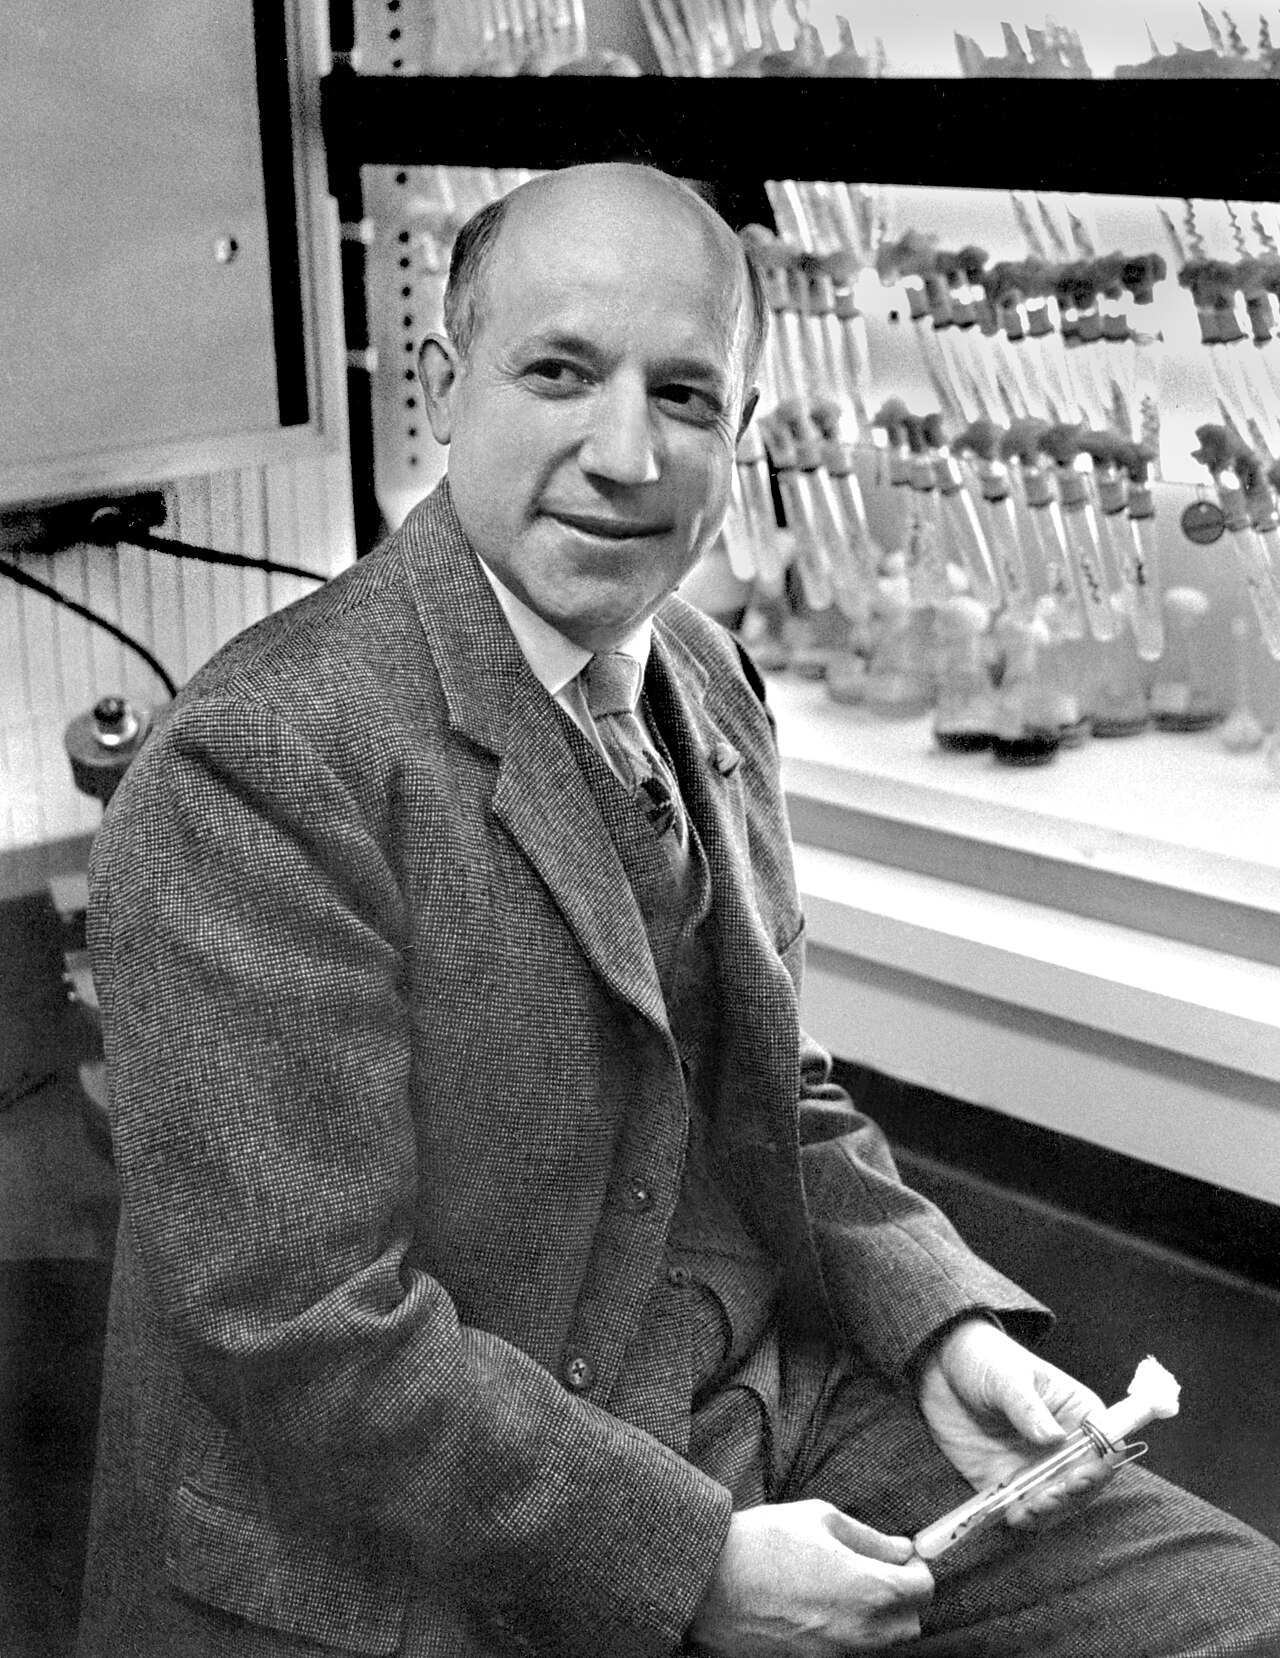
\includegraphics[width=0.26\linewidth]{images/book3/calvin.jpg}

{\small Melvin Calvin (1911--1997), who with Benson traced the path of
carbon from $\mathrm{CO_2}$ to sugar with radioactive carbon and paper
chromatography. Photograph: Lawrence Berkeley Laboratory, public
domain.}
\end{omfigure}

\begin{omfigure}
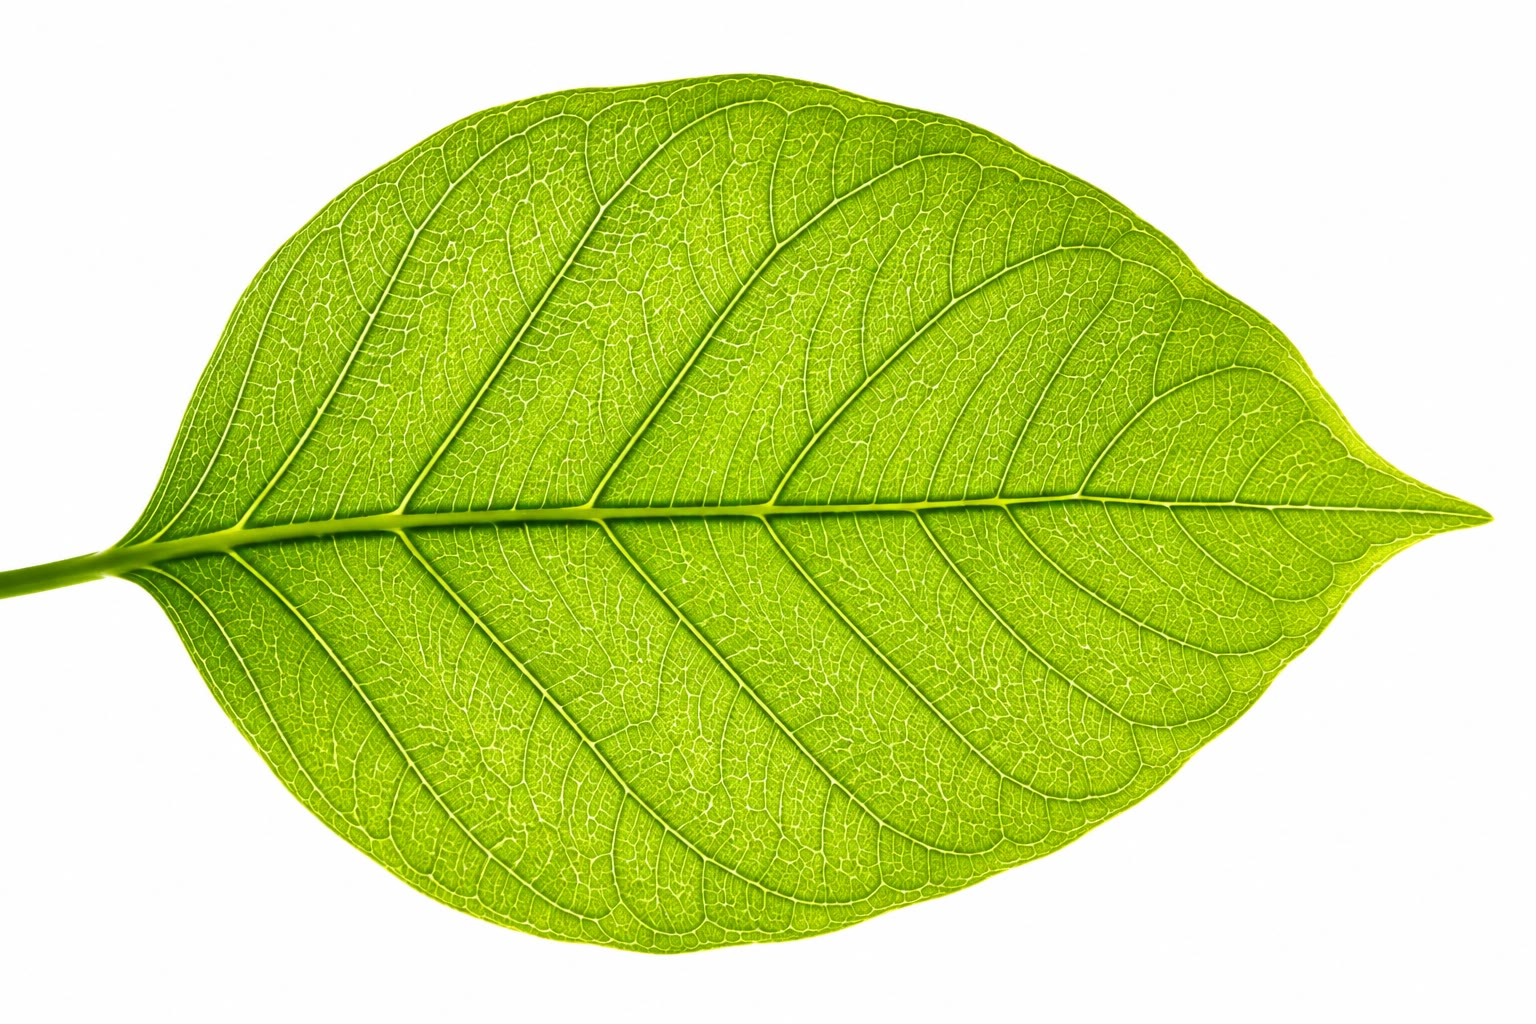
\includegraphics[width=0.6\linewidth]{images/book3/ai/b3-14-leaf-backlit.jpg}

{\small A \omterm{def:b1:flowering-plant-organization:organs}{leaf} against the sun: the light it absorbs drives, in every
\omterm{def:b1:photosynthesis:chloroplast}{chloroplast} of its palisade \omterm{def:b1:cell-unit-of-life:cell}{cells}, the splitting of water and the
fixation of the carbon dioxide that entered through its \omterm{def:b1:flowering-plant-organization:tissues}{stomata}.}
\end{omfigure}

\begin{method}[Balancing a photosynthetic budget]\label{met:b1:photosynthesis:budget}
\begin{enumerate}
  \item Count carbons: each $\mathrm{CO_2}$ fixed yields one carbon of
        product; one glucose needs six turns of \omterm{def:b1:photosynthesis:fixation}{RuBisCO}.
  \item Count carriers: each turn costs 3 \omterm{def:b1:water-small-molecules:atp}{ATP} and 2 NADPH (9 and 6
        per G3P); one glucose costs 18 \omterm{def:b1:water-small-molecules:atp}{ATP} and 12 NADPH.
  \item Count photons: the linear flow gives 2 NADPH and about 3 \omterm{def:b1:water-small-molecules:atp}{ATP}
        per $\mathrm{O_2}$, for 8 photons (4 per \omterm{def:b1:photosynthesis:zscheme}{photosystem}); 12 NADPH
        need 6 $\mathrm{O_2}$ and 48 photons; the extra \omterm{def:b1:water-small-molecules:atp}{ATP} comes from
        cyclic flow (a few more photons). About 8 photons per
        $\mathrm{CO_2}$: the quantum requirement.
  \item Count energy: a mole of \qty{680}{nm} photons is \qty{176}{kJ};
        48 photons are \qty{8450}{kJ} for \qty{2870}{kJ} stored in
        glucose: \qty{34}{\%} at best, before any loss to reflection,
        respiration and the fraction of the spectrum not absorbed.
\end{enumerate}
\end{method}

\section{Photorespiration, C4 and CAM}

\begin{proposition}[RuBisCO's flaw]\label{prop:b1:photosynthesis:photorespiration}
\index{photorespiration}
\omterm{def:b1:photosynthesis:fixation}{RuBisCO} also accepts $\mathrm{O_2}$ in place of $\mathrm{CO_2}$: the
oxygenation of RuBP yields one 3-PGA and one two-carbon phosphoglycolate,
which the \omterm{def:b1:cell-unit-of-life:cell}{cell} must salvage through a costly route across three
\omterm{def:b1:cell-unit-of-life:prokeuk}{organelles} that releases $\mathrm{CO_2}$ and consumes \omterm{def:b1:water-small-molecules:atp}{ATP} ---
\emph{photorespiration}. The \omterm{def:b1:enzymes:enzyme}{enzyme} discriminates poorly (about
\qty{80}{} to 1 in favour of $\mathrm{CO_2}$ at equal concentrations),
and in air $\mathrm{O_2}$ is five hundred times more abundant than
$\mathrm{CO_2}$; at \qty{25}{\celsius} a quarter of the fixations are
wasted, more in hot, dry weather when \omterm{def:b1:flowering-plant-organization:tissues}{stomata} close and $\mathrm{CO_2}$
falls inside the \omterm{def:b1:flowering-plant-organization:organs}{leaf}. \omterm{def:b1:photosynthesis:fixation}{RuBisCO}, evolved when the air had no oxygen, is
also slow (three turnovers per second) and is compensated by
abundance: it is the most plentiful \omterm{def:b1:proteins:peptide}{protein} on Earth, half the soluble
\omterm{def:b1:proteins:peptide}{protein} of a \omterm{def:b1:flowering-plant-organization:organs}{leaf}.
\end{proposition}

\begin{definition}[C4 and CAM plants]\label{def:b1:photosynthesis:c4cam}
\index{C4 plant}\index{CAM plant}
\emph{C4 plants} (maize, sugar cane, sorghum, many tropical grasses)
seal the leak by concentrating $\mathrm{CO_2}$: in the mesophyll \omterm{def:b1:cell-unit-of-life:cell}{cells}
an \omterm{def:b1:enzymes:enzyme}{enzyme} with no affinity for $\mathrm{O_2}$ (PEP carboxylase) fixes
bicarbonate into a four-carbon acid, which is shuttled into the
\emph{bundle-sheath} \omterm{def:b1:cell-unit-of-life:cell}{cells} around the veins and decarboxylated there,
raising the $\mathrm{CO_2}$ around \omterm{def:b1:photosynthesis:fixation}{RuBisCO} tenfold and suppressing
oxygenation --- at a cost of two extra \omterm{def:b1:water-small-molecules:atp}{ATP} per $\mathrm{CO_2}$. The two
\omterm{def:b1:cell-unit-of-life:cell}{cell} types form the \emph{Kranz} (``wreath'') anatomy. \emph{CAM plants}
(cacti, pineapple, agaves) separate the same two steps in time rather
than space: they open their \omterm{def:b1:flowering-plant-organization:tissues}{stomata} at night, store $\mathrm{CO_2}$ as
malic acid in the \omterm{def:b1:eukaryotic-cell:plantcell}{vacuole}, and release it to \omterm{def:b1:photosynthesis:fixation}{RuBisCO} by day behind
closed \omterm{def:b1:flowering-plant-organization:tissues}{stomata}, losing a tenth of the water a C3 plant loses per
carbon fixed.
\end{definition}

\begin{omfigure}
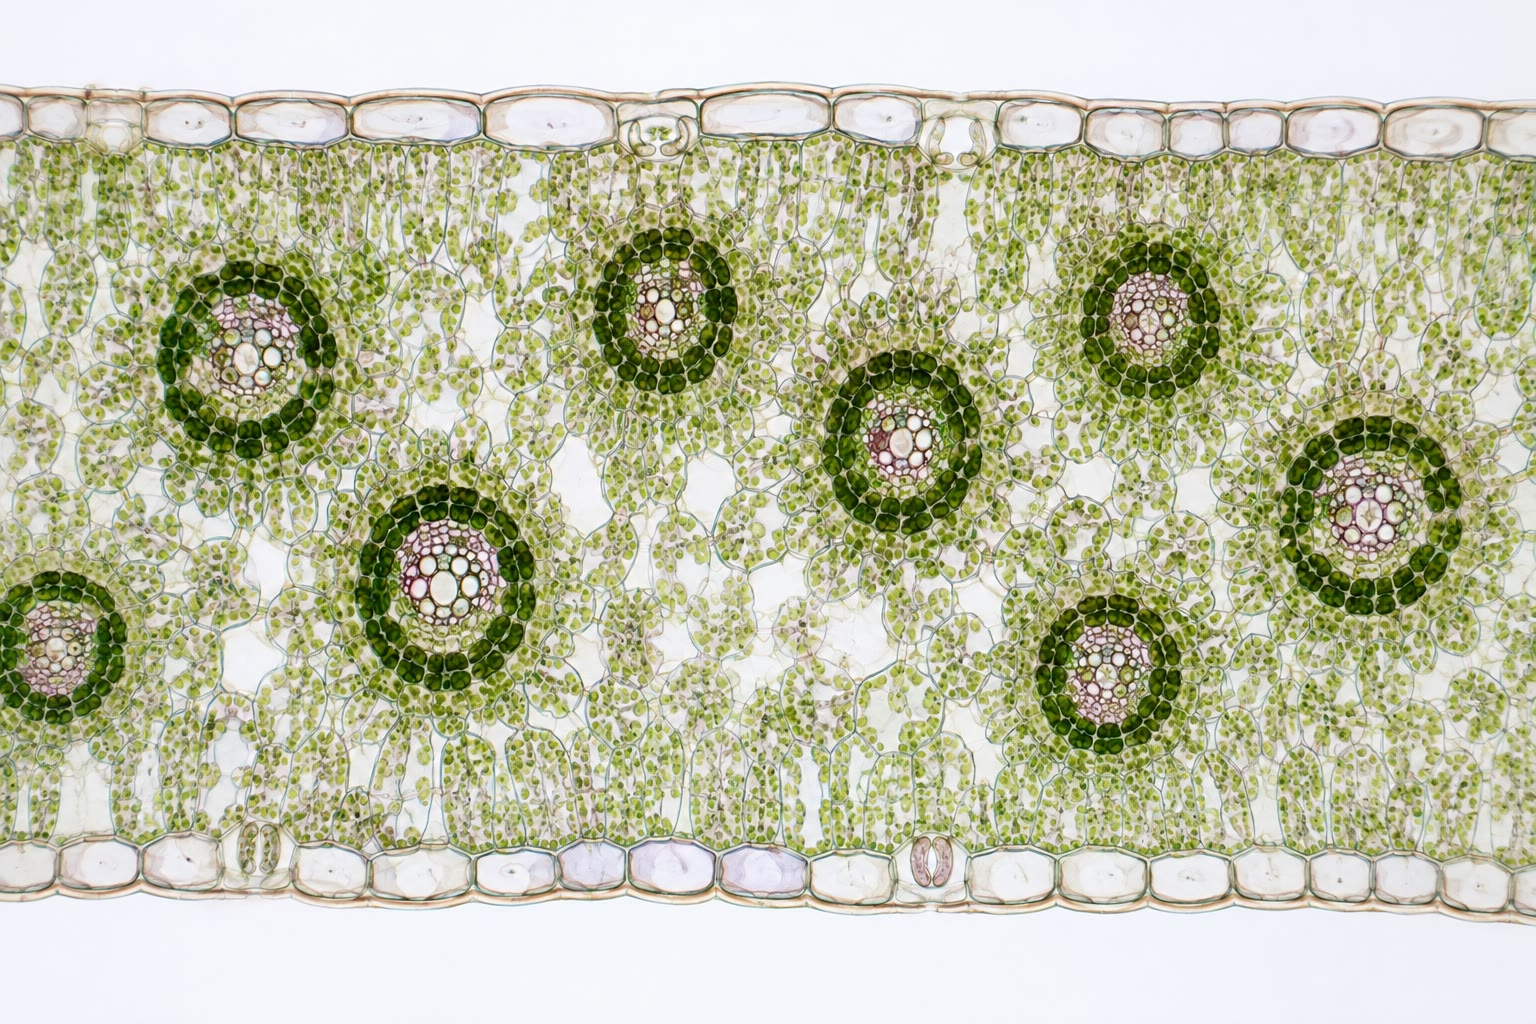
\includegraphics[width=0.6\linewidth]{images/book3/ai/b3-14-maize-kranz.jpg}

{\small Kranz anatomy in a maize \omterm{def:b1:flowering-plant-organization:organs}{leaf}: each vein is wreathed by
large bundle-sheath \omterm{def:b1:cell-unit-of-life:cell}{cells} packed with \omterm{def:b1:eukaryotic-cell:plastid}{chloroplasts}, themselves ringed
by mesophyll \omterm{def:b1:cell-unit-of-life:cell}{cells}. $\mathrm{CO_2}$ is captured in the outer ring and
delivered, concentrated, to \omterm{def:b1:photosynthesis:fixation}{RuBisCO} in the inner one.}
\end{omfigure}

\begin{example}[Which plant where]\label{ex:b1:photosynthesis:where}
At \qty{20}{\celsius} in moist air a C3 wheat \omterm{def:b1:flowering-plant-organization:organs}{leaf} and a C4 maize \omterm{def:b1:flowering-plant-organization:organs}{leaf}
fix carbon at similar rates, and the maize pays two \omterm{def:b1:water-small-molecules:atp}{ATP} more per
carbon. At \qty{35}{\celsius} in dry air the wheat loses a third of
its fixation to photorespiration while the maize loses none: C4 grasses
dominate hot open country, C3 plants the cool and shaded. A cactus
fixes slowly by either standard but survives where the others would
die of thirst.
\end{example}

\section{Autotrophy}

\begin{definition}[Autotrophy]\label{def:b1:photosynthesis:autotrophy}
An \omterm{def:b1:organism-environment:organism}{organism} is \emph{autotrophic}\index{autotrophy} when it builds its
organic matter from $\mathrm{CO_2}$ (\cref{ch:b1:organism-environment}).
It needs a source of energy and a source of electrons.
\emph{\omterm{def:b1:organism-environment:trophy}{Photoautotrophs}} take energy from light: plants, algae and
cyanobacteria take their electrons from water and release oxygen
(\emph{oxygenic}); purple and green bacteria take them from hydrogen
sulfide or organic acids and release none. \emph{\omterm{def:b1:organism-environment:trophy}{Chemoautotrophs}}
take both energy and electrons from the oxidation of inorganic
compounds --- ammonia, nitrite, sulfide, hydrogen, ferrous iron --- with
no light at all: the nitrifying bacteria of the soil, and the bacteria
that feed the ecosystems of deep-sea vents. All use the \omterm{def:b1:photosynthesis:fixation}{Calvin cycle},
or a related cycle, to fix the carbon; all reduce it with NADPH and
pay with \omterm{def:b1:water-small-molecules:atp}{ATP}; they differ only in where the \omterm{def:b1:water-small-molecules:atp}{ATP} and the electrons come
from.
\end{definition}

\begin{example}[The global budget]\label{ex:b1:photosynthesis:global}
Photosynthesis fixes about \qty{120}{Gt} of carbon a year on land and
\qty{50}{Gt} in the oceans, half of it by single-celled algae and
cyanobacteria invisible to the eye; it turns over the carbon dioxide
of the atmosphere every seven years and its oxygen every two thousand.
The oxygen came the same way: for two billion years cyanobacteria
released it into an atmosphere that had none, and every aerobic
\omterm{def:b1:organism-environment:organism}{organism}, from the \omterm{def:b1:eukaryotic-cell:mitochondrion}{mitochondrion} up, is built on the leak of one
\omterm{def:b1:enzymes:enzyme}{enzyme} system that splits water.
\end{example}

\section{Exercises}

\begin{exercise}[$\star$]\label{exo:b1:photosynthesis:1}
Name the three membrane systems of the \omterm{def:b1:photosynthesis:chloroplast}{chloroplast} and say where the
\omterm{prop:b1:photosynthesis:lightreactions}{light reactions} and the \omterm{def:b1:photosynthesis:fixation}{Calvin cycle} take place.
\end{exercise}

\begin{exercise}[$\star$]\label{exo:b1:photosynthesis:2}
Write the equation of the \omterm{prop:b1:photosynthesis:lightreactions}{light reactions} and say where the released
oxygen comes from, with the evidence.
\end{exercise}

\begin{exercise}[$\star$]\label{exo:b1:photosynthesis:3}
Name the three stages of the \omterm{def:b1:photosynthesis:fixation}{Calvin cycle} and the number of \omterm{def:b1:water-small-molecules:atp}{ATP} and
NADPH consumed per $\mathrm{CO_2}$ fixed.
\end{exercise}

\begin{exercise}[$\star$]\label{exo:b1:photosynthesis:4}
From the spectra figure, at which wavelengths does \omterm{def:b1:photosynthesis:pigments}{chlorophyll} $a$
absorb most, and why is the action spectrum higher than the
\omterm{def:b1:photosynthesis:pigments}{chlorophyll} absorption around \qty{500}{nm}?
\end{exercise}

\begin{exercise}[$\star\star$]\label{exo:b1:photosynthesis:5}
Explain the Emerson enhancement effect and what it revealed about the
organisation of the \omterm{prop:b1:photosynthesis:lightreactions}{light reactions}.
\end{exercise}

\begin{exercise}[$\star\star$]\label{exo:b1:photosynthesis:6}
A proton-motive force of \qty{0.18}{V} corresponds to how much \omterm{prop:b1:water-small-molecules:gibbs}{free
energy} per mole of protons ($F = \qty{96500}{C/mol}$)? How many
protons must flow to make one \omterm{def:b1:water-small-molecules:atp}{ATP} at \qty{50}{kJ/mol}? Compare with
the four the synthase uses.
\end{exercise}

\begin{exercise}[$\star\star$]\label{exo:b1:photosynthesis:7}
Jagendorf's \omterm{def:b1:photosynthesis:chloroplast}{thylakoids} made \omterm{def:b1:water-small-molecules:atp}{ATP} in the dark after an acid bath.
Explain what this proves and what it does not, and predict the result
if an uncoupler is added before the transfer.
\end{exercise}

\begin{exercise}[$\star\star$]\label{exo:b1:photosynthesis:8}
Follow the carbon: starting from 3 RuBP (15 carbons) and 3
$\mathrm{CO_2}$, count carbons through 3-PGA, G3P, the exported G3P and
the regenerated RuBP, and verify the balance.
\end{exercise}

\begin{exercise}[$\star\star$]\label{exo:b1:photosynthesis:9}
In Calvin's experiment, RuBP rises and 3-PGA falls when $\mathrm{CO_2}$
is removed; 3-PGA rises and RuBP falls when the light is switched off.
Explain both from the cycle.
\end{exercise}

\begin{exercise}[$\star\star\star$]\label{exo:b1:photosynthesis:10}
Compute the energy of a mole of \qty{680}{nm} photons ($h =
\qty{6.63e-34}{J.s}$, $c = \qty{3.0e8}{m/s}$, $N_A = \num{6.02e23}$),
the energy of the 48 photons needed per glucose, and the efficiency
of storing \qty{2870}{kJ/mol}. Why is the efficiency of a whole crop,
about \qty{1}{\%} of the sunlight, so much lower?
\end{exercise}

\begin{exercise}[$\star\star\star$]\label{exo:b1:photosynthesis:11}
At \qty{25}{\celsius} in air \omterm{def:b1:photosynthesis:fixation}{RuBisCO} oxygenates once for every three
carboxylations; each oxygenation releases half a $\mathrm{CO_2}$ in
salvage and costs \omterm{def:b1:water-small-molecules:atp}{ATP}. Compute the net carbon fixed per 100
carboxylations and the fraction lost. A \omterm{def:b1:photosynthesis:c4cam}{C4 plant} avoids the loss but
spends 2 extra \omterm{def:b1:water-small-molecules:atp}{ATP} per $\mathrm{CO_2}$: at what fraction of loss does
the C4 design pay, if one \omterm{def:b1:water-small-molecules:atp}{ATP} is worth about a tenth of a $\mathrm{CO_2}$
fixed?
\end{exercise}

\begin{exercise}[$\star\star\star$]\label{exo:b1:photosynthesis:12}
``Photosynthesis is respiration run backward.'' Discuss in a paragraph,
comparing the chemiosmotic mechanism, the direction of electron flow,
the carriers and the cycles, and saying where the analogy holds and
where it fails.
\end{exercise}

\section{Problem: The Price of a Molecule of Glucose}

\begin{problem}[{Weekend problem --- photons counted, electrons and
protons followed through the thylakoid, ATP and NADPH reckoned and
spent, a leaf's daily harvest weighed, ending on the energy efficiency
of photosynthesis}]
\label{pb:b1:photosynthesis:1}
Constants: $h = \qty{6.63e-34}{J.s}$, $c = \qty{3.00e8}{m/s}$,
$N_A = \num{6.02e23}$, $F = \qty{96500}{C/mol}$, $R = \qty{8.314}{J.mol^{-1}.K^{-1}}$,
$T = \qty{298}{K}$. \omterm{prop:b1:water-small-molecules:gibbs}{Free energy} of glucose combustion
\qty{2870}{kJ/mol}; \omterm{def:b1:water-small-molecules:atp}{ATP} synthesis in the \omterm{def:b1:photosynthesis:chloroplast}{chloroplast} costs
\qty{50}{kJ/mol}; NADPH holds \qty{220}{kJ/mol} of reducing power.

\medskip
\noindent\textbf{Part I --- Photons and electrons.}
\begin{enumerate}
  \item Compute the energy of one photon of \qty{680}{nm} and of a
        mole of them.
  \item Compute the energy of a mole of \qty{700}{nm} photons and of
        \qty{450}{nm} photons. Why does blue light give no more
        photosynthesis per photon than red?
  \item How many photons of \qty{680}{nm} carry one joule?
  \item Moving one electron from water ($E'_0 = \qty{+0.82}{V}$) to
        $\mathrm{NADP^+}$ ($E'_0 = \qty{-0.32}{V}$) requires how much
        \omterm{prop:b1:water-small-molecules:gibbs}{free energy} per mole of electrons ($\Delta G = -nF\Delta E$)?
  \item Two photons are used per electron (one in each \omterm{def:b1:photosynthesis:zscheme}{photosystem}).
        Compute the energy supplied per mole of electrons and the
        fraction of it stored in the redox change.
  \item How many electrons, and hence how many photons, are needed to
        make one $\mathrm{O_2}$ and two NADPH?
  \item How many photons per glucose, if 12 NADPH are needed?
\end{enumerate}

\medskip
\noindent\textbf{Part II --- Protons and \omterm{def:b1:water-small-molecules:atp}{ATP}.}
For each $\mathrm{O_2}$ released, four protons are freed in the lumen
by water splitting and eight are pumped by the cytochrome $b_6f$
complex; the \omterm{thm:b1:photosynthesis:chemiosmosis}{ATP synthase} uses \qty{4}{H^+} per \omterm{def:b1:water-small-molecules:atp}{ATP}. The lumen is at
pH 5 and the \omterm{def:b1:photosynthesis:chloroplast}{stroma} at pH 8; the \omterm{def:b1:membranes-transport:potential}{membrane potential} across the
\omterm{def:b1:photosynthesis:chloroplast}{thylakoid} is negligible.
\begin{enumerate}[resume]
  \item Compute the proton-motive force from the pH difference, in
        volts ($\Delta\mu = 2.303\,RT\,\Delta\mathrm{pH}/F$), and the
        \omterm{prop:b1:water-small-molecules:gibbs}{free energy} per mole of protons.
  \item Compute the protons delivered to the lumen per $\mathrm{O_2}$
        and the \omterm{def:b1:water-small-molecules:atp}{ATP} they can make.
  \item Compute the \omterm{def:b1:water-small-molecules:atp}{ATP} made per glucose by linear flow (6
        $\mathrm{O_2}$), and compare with the 18 the \omterm{def:b1:photosynthesis:fixation}{Calvin cycle}
        needs. How is the shortfall made up?
  \item Compute the \omterm{prop:b1:water-small-molecules:gibbs}{free energy} available from the protons per \omterm{def:b1:water-small-molecules:atp}{ATP}
        (\qty{4}{H^+}) and the efficiency of the synthase.
  \item The lumen of a \omterm{def:b1:photosynthesis:chloroplast}{chloroplast} has a volume of about
        \qty{1}{\micro m^3}. How many free protons does it hold at pH
        5? Compare with the roughly $10^5$ protons that pass through
        the synthases each second, and conclude what \omterm{def:b1:water-small-molecules:buffer}{buffers} the
        lumen.
\end{enumerate}

\medskip
\noindent\textbf{Part III --- Sugar.}
\begin{enumerate}[resume]
  \item Write the energy stored per glucose as 18 \omterm{def:b1:water-small-molecules:atp}{ATP} $\times$
        \qty{50}{kJ} plus 12 NADPH $\times$ \qty{220}{kJ}, and compare
        it with the \qty{2870}{kJ} of glucose. Where does the
        difference go?
  \item Compute the energy of the 48 photons of question 6 and the
        efficiency of photosynthesis from photon to glucose.
  \item Only \qty{45}{\%} of sunlight is in the wavelengths the
        pigments absorb, and of that a tenth is reflected or
        transmitted. Compute the efficiency from incident sunlight to
        glucose, before respiration.
  \item A \omterm{def:b1:flowering-plant-organization:organs}{leaf} of \qty{50}{cm^2} receives \qty{400}{W/m^2} of sunlight
        for \qty{10}{h}. Compute the energy received and, at the
        efficiency of question 14, the glucose made in grams
        (\qty{180}{g/mol}).
  \item The \omterm{def:b1:flowering-plant-organization:organs}{leaf} respires \qty{40}{\%} of that glucose to stay alive.
        What is its net gain, in grams of glucose and in grams of
        carbon?
  \item A crop reaches \qty{1}{\%} overall efficiency in a season. List
        three losses, beyond those already counted, that separate the
        \omterm{def:b1:flowering-plant-organization:organs}{leaf}'s figure from the crop's.
\end{enumerate}

\medskip
\noindent\textbf{Part IV --- The leak.}
\omterm{def:b1:photosynthesis:fixation}{RuBisCO} in air at \qty{25}{\celsius} performs one oxygenation per three
carboxylations; each oxygenation costs the equivalent of half a
$\mathrm{CO_2}$ fixed and 3.5 \omterm{def:b1:water-small-molecules:atp}{ATP}.
\begin{enumerate}[resume]
  \item Per 100 carboxylations, compute the oxygenations, the carbon
        lost and the net carbon gained.
  \item Compute the \omterm{def:b1:water-small-molecules:atp}{ATP} spent on salvage per 100 carboxylations and
        the total \omterm{def:b1:water-small-molecules:atp}{ATP} per net carbon gained (\omterm{def:b1:photosynthesis:fixation}{Calvin cycle} 3 \omterm{def:b1:water-small-molecules:atp}{ATP} per
        carboxylation plus salvage).
  \item A \omterm{def:b1:photosynthesis:c4cam}{C4 plant} has no oxygenation but spends 2 extra \omterm{def:b1:water-small-molecules:atp}{ATP} per
        $\mathrm{CO_2}$ delivered. Compute its \omterm{def:b1:water-small-molecules:atp}{ATP} per net carbon and
        compare.
  \item At \qty{35}{\celsius} the oxygenation ratio rises to one in
        two. Recompute the C3 figures and say which design wins.
  \item Explain why raising the $\mathrm{CO_2}$ of a greenhouse to
        three times the atmospheric value raises the yield of C3
        crops (tomato, wheat) but barely that of C4 crops (maize).
  \item A C3 \omterm{def:b1:flowering-plant-organization:organs}{leaf} loses about 250 water molecules per $\mathrm{CO_2}$
        fixed, a \omterm{def:b1:photosynthesis:c4cam}{CAM plant} about 25. Compute the water each loses to
        fix \qty{1}{g} of carbon.
  \item State the result: the quantum requirement per $\mathrm{CO_2}$,
        the efficiency from photon to glucose, and the efficiency from
        sunlight to net \omterm{def:b1:flowering-plant-organization:organs}{leaf} sugar.
\end{enumerate}
\end{problem}
